\documentclass[11pt]{article}
\usepackage{titlesec}

\setcounter{secnumdepth}{4}

\parindent 0px % no automatic indentation

\usepackage{amsmath,amssymb,amstext,amsthm,amsfonts}
\usepackage{float}
\usepackage[shortlabels]{enumitem}
\usepackage[a4paper,lmargin={2cm},rmargin={2cm},tmargin={2.5cm},bmargin = {2.5cm},headheight = {4cm}]{geometry}

\usepackage[utf8]{inputenc}
\usepackage[T1]{fontenc}
%\usepackage[ngerman]{babel}
\usepackage{lmodern}
\usepackage{color}
\usepackage{xcolor}
\usepackage{colortbl}
\usepackage{graphicx}
\usepackage{listings}
\usepackage{xspace}
\usepackage{empheq}
\usepackage{mdframed}
\usepackage{changepage}
%\usepackage{hanging}
\usepackage{romanbar}
\usepackage{mathtools}
\usepackage[hidelinks]{hyperref}

\usepackage[headsepline]{scrlayer-scrpage} 
\pagestyle{scrheadings} 
\usepackage{titling}
\usepackage{cancel}
\usepackage{booktabs}
\usepackage{algorithm}
\usepackage{algpseudocode}

\usepackage{listings}
\usepackage{xcolor} % Optional, for coloring code
\usepackage{multirow}

\lstset{
  language=SQL,  % Setting the language
  basicstyle=\ttfamily\small, % The default font size and style of the code
  showspaces=false, % Show spaces adding particular underscores
  showstringspaces=false, % Underline spaces within strings only
  showtabs=false, % Show tabs within strings adding particular underscores
  %frame=single, % Adds a frame around the code
  tabsize=2, % Sets default tabsize to 2 spaces
  captionpos=b, % Sets the caption-position to bottom
  breaklines=true,  % Sets automatic line breaking
  breakatwhitespace=false, % Sets if automatic breaks should only happen at whitespace
  commentstyle=\color{gray}, % Comment style
  keywordstyle=\color{blue}, % Keyword style
  stringstyle=\color{red}  % String literal style
}

\pagestyle{plain}

% MACROS
\newcommand{\ind}{\perp\!\!\!\!\perp} 


\title{Database Systems}
\author{Michael Sigg}
\date{\today}

\ohead{\theauthor}
\ihead{Database Systems, Spring 24}



\begin{document}
\maketitle
\tableofcontents

\newpage

\section{Database Systems}
\subsection{Definitions}
\begin{itemize}[label=\(\rhd\)]
    \item \textbf{Database (DB)}: A collection of related data
    \item \textbf{Database Management System (DBMS)}: A software package to facilitate the creation/maintenance/querying of databases
    \item \textbf{Database System (DBS)}: DB + DBMS
    \item \textbf{Meta Data}: Information about the structure of the DB
\end{itemize}

\begin{figure}[H]
\centering
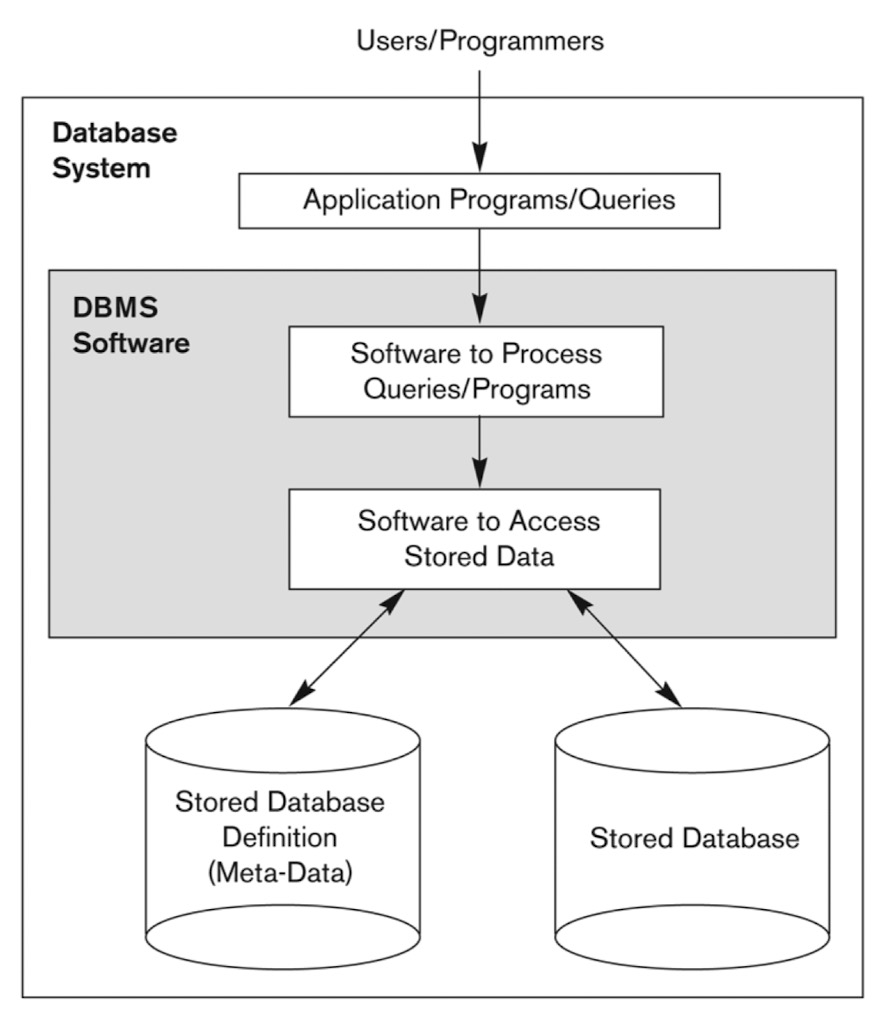
\includegraphics[width=0.8\textwidth]{images/Screenshot 2024-05-01 at 17.02.18.jpg}
\caption{Database System}
\end{figure}

A DBMS offers two types of languages:
\begin{itemize}[label=\(\rhd\)]
    \item[1.] data definition language (\textbf{DDL}) to create and drop tables, etc.
    \item[2.] data manipulation language (\textbf{DML}) to select, insert, delete, and update data 
    \item SQL offers both.
\end{itemize}

\textbf{\underline{Functionality of Database Systems}}
\bigskip
Typical DBMS functionality:
\begin{itemize}[label=\(\rhd\)]
    \item \textbf{Define} a particular database in terms of its data types, structures, and constraints
    \item \textbf{Construct} or \textbf{load} the initial database contents on a persistent storage medium
    \item \textbf{Manipulating} the database:
    \begin{itemize}[label=\(\rhd\)]
        \item Retrieval: querying, generating reports
        \item Modification: insertions, deletions and updates to its content
    \end{itemize}
    \item \textbf{Sharing} by a set of concurrent users and application programs while, at the same time, keeping all data valid and consistent.
\end{itemize}

\textbf{\underline{Redundancy}}
\bigskip
A key goal of database design is to avoid redundancy. \textbf{Redundancy} is present if information is stored multiple times. Redundancy leads to update anomalies and inconsistent data. The term \textbf{controlled redundancy} is used if duplication of information is allowed and if the duplication is controlled by the DBMS.

\subsection{Main Characteristics of Database Systems}

\textbf{\underline{DBMS Architecture}}

\begin{figure}[H]
\centering
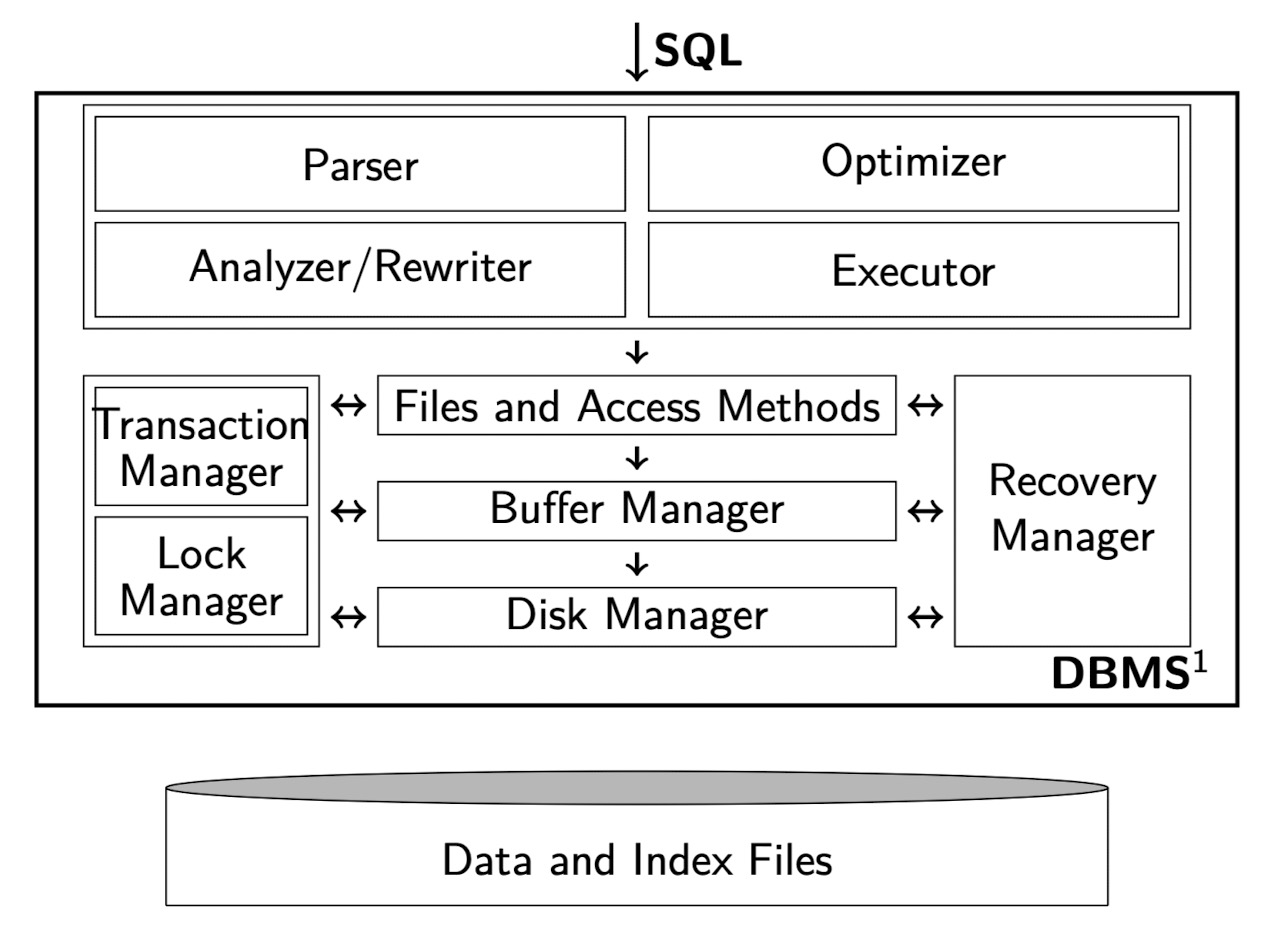
\includegraphics[width=0.8\textwidth]{images/Screenshot 2024-05-01 at 17.25.40.jpg}
\caption{DBMS Architecture}
\end{figure}

\subsection{Summary}
\begin{itemize}[label=\(\rhd\)]
    \item Data models, schema, instances
    \begin{itemize}[label=\(\rhd\)]
        \item \textbf{data model} = structures + constraints + operations
        \item \textbf{schema} = intension; schema consists of structures and constraints; schema changes infrequently 
        \item \textbf{relation instance} = relation = extension; relation instance is the actual data that is compatible with the schema; changes often
    \end{itemize}
    \item Key characteristics of database systems
    \begin{itemize}[label=\(\rhd\)]
        \item \textbf{controlled redundancy}: database systems is aware of redundancy and provides support for updates that could violate the consistency of the data
        \item \textbf{data independence}: separation of program and data; makes it possible to, e.g., reorganize internal schema without changing conceptual schema
        \item \textbf{data abstraction}: high level query language that is independent of storage structure
        \item \textbf{data dictionary} (metadata) that stores information about the database itself (self-describing)
    \end{itemize}
\end{itemize}

\section{The Relational Model}
\subsection{The Relational Model}

\textbf{\underline{Relation Schema}}
\bigskip
\begin{itemize}[label=\(\rhd\)]
    \item A \textbf{relation schema} R, denoted by $R(A_1,A_2,...,A_n)$, is made up of a relation name and a list of attributes.
    \item $attr(R)$ denotes the set of attributes of relation with name 
    \begin{itemize}[label=\(\rhd\)]
        \item[] $R$: $attr(Customer) = \underbrace{\{CustName, CustStreet, CustCity\}}_\text{Set}$
    \end{itemize}
\end{itemize}

\textbf{\underline{Attribute}}
\bigskip
\begin{itemize}[label=\(\rhd\)]
    \item The set of allowed values for each attribute is called the \textbf{domain} of the attribute
    \item Attribute values are required to be \textbf{atomic}; that is, indivisible
\end{itemize}

\textbf{\underline{Example of a Relation}}
\bigskip
\begin{figure}[H]
\centering
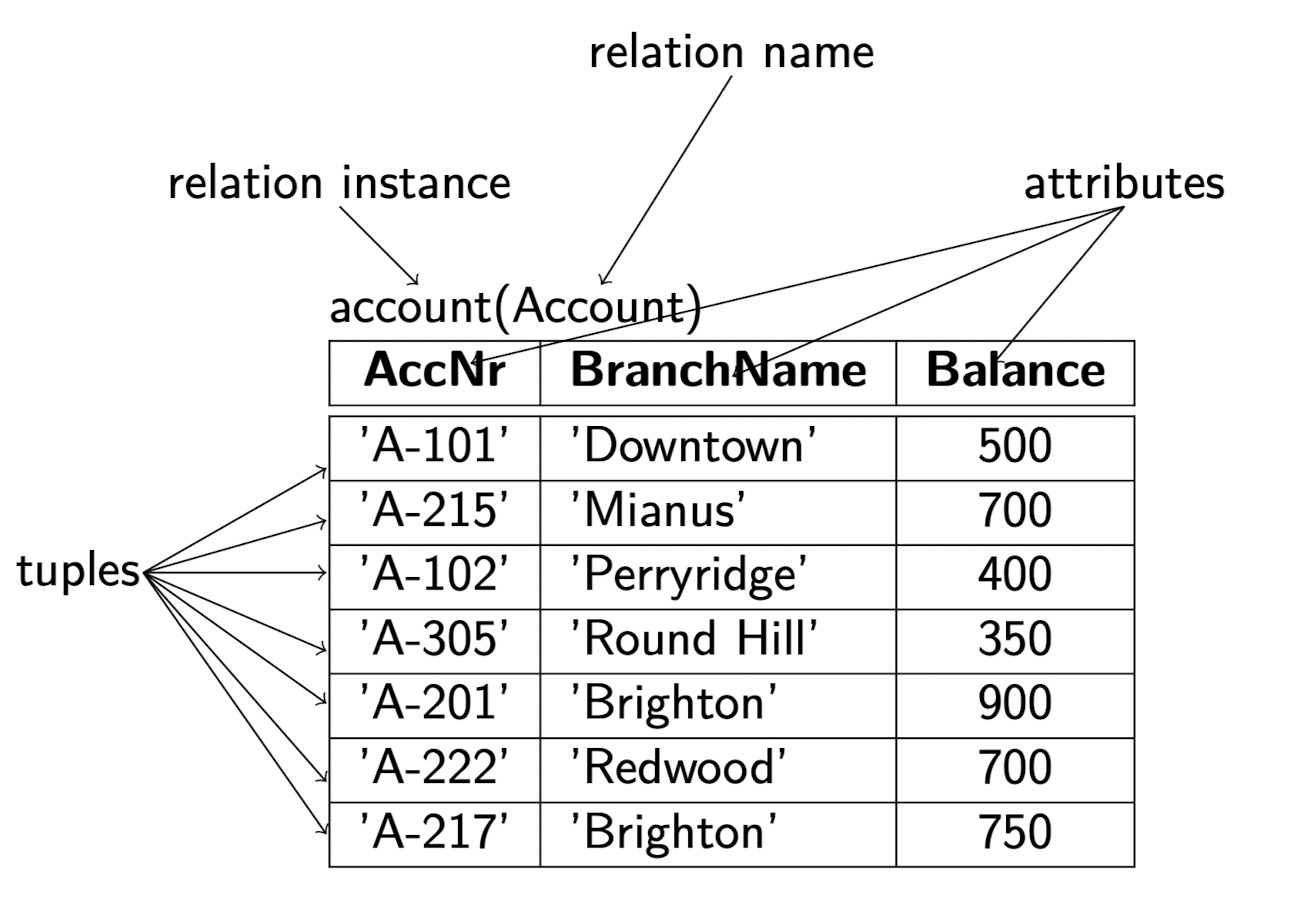
\includegraphics[width=0.8\textwidth]{images/Screenshot 2024-05-01 at 17.58.27.jpg}
\caption{Relation Example}
\end{figure}

\textbf{\underline{Characteristics of Relations}}
\bigskip
\begin{itemize}[label=\(\rhd\)]
    \item Relations are \textbf{unordered}, i.e., the order of tuples is irrelevant
\end{itemize}

\textbf{\underline{Database}}
\begin{itemize}[label=\(\rhd\)]
    \item A database consists of multiple relations
\end{itemize}

\textbf{\underline{Summary of the Relational Data Model}}
\begin{itemize}[label=\(\rhd\)]
    \item A \textbf{domain} $D$ is a set of atomic data values.
    \begin{itemize}[label=\(\rhd\)]
        \item phone numbers, names, grades, birthdates, departments
        \item each domain includes the special value \texttt{null}
    \end{itemize}
    \item With each domain a \textbf{data type} or format is specified.
    \begin{itemize}[label=\(\rhd\)]
        \item 5 digit integers, yyyy-mm-dd, characters
    \end{itemize}
    \item An \textbf{attribute} $A_i$ describes the role of a domain in a relation schema
    \begin{itemize}[label=\(\rhd\)]
        \item PhoneNr, Age, DeptName
    \end{itemize}
    \item A \textbf{relation schema} $R(A_1,...,A_n)$ is made up of a relation name $R$ and a list of attributes
    \begin{itemize}[label=\(\rhd\)]
        \item $Employee(Name,Dept,Salary),\ Departement(DName, Manager, Address)$
    \end{itemize}
    \item A \textbf{tuple} $t$ is an ordered list of values $t=(v_1,...,v_n)$ with $v_i \in dom(A_i)$
    \begin{itemize}[label=\(\rhd\)]
        \item $t=('Tom','SE',23K)$
    \end{itemize}
    \item A \textbf{relation} $r\subseteq D_1 \times ... \times D_n$ over schema $R(A_1,...,A_n)$ is a set of n-ary tuples
    \begin{itemize}[label=\(\rhd\)]
        \item $r= \{('Tom','SE',23K),('Lene','DB',33K)\}\subseteq Names \times Departments \times Integer$
        \item $s=\{('SE', 'Tom','Boston'),('DB','Lena','Tucson')\}$
    \end{itemize}
    \item A \textbf{database} $DB$ is a set of relations
    \begin{itemize}[label=\(\rhd\)]
        \item $DB=\{r,s\}$
    \end{itemize}
\end{itemize}

\textbf{\underline{Constraints}}
\bigskip
Key Constraints \label{keyConstraints}
\begin{itemize}[label=\(\rhd\)]
    \item Let $K\subseteq attr(R)$
    \item $K$ is a \textbf{superkey} of $R$ if values for $K$ are sufficient to identify a unique tuple of each possible relation $r$
    \item Superkey are not minimal
    \item $K$ is a \textbf{candidate key} if $K$ is a \textit{superkey} and $K$ is minimal
    \item \textbf{Primary key}: a candidate key chosen as the principal means of identifying tuples within a relation
\end{itemize}
Entity constraints
\begin{itemize}[label=\(\rhd\)]
    \item The entity constraint requires that the primary key attributes of each relation may not have \texttt{null} values
\end{itemize}
\textbf{\underline{Referential Integrity}}
\bigskip
\begin{itemize}[label=\(\rhd\)]
    \item A relation schema may have an attribute that corresponds to the primary key of a relation. The attribute is called a \textbf{foreign key}.
\end{itemize}

\subsection{Basic Relational Algebra Operators}

\textbf{\underline{Basic Operators}}:
\begin{itemize}[label=\(\rhd\)]
    \item Select $\sigma$
    \item Project $\pi$
    \item Union $\cup$
    \item Set difference $-$
    \item Cartesian product $\times$
    \item Rename $\rho$
\end{itemize}

Relational algebra is a procedural language, i.e., order of operation matters

\subsubsection{Select Operator}
\begin{itemize}[label=\(\rhd\)]
    \item \textbf{Notation}: $\sigma_p(r)$
    \item $p$ is called the \textbf{selection predicate}
    \item \textbf{Definition}: $t\in \sigma_p(r) \Leftrightarrow t \in r \land p(t)$
    \item $p$ is a condition in propositional calculus consisting of \textbf{terms} connected by: $\land$ (\textbf{and}), $\lor$ (\textbf{or}), $\lnot$ (\textbf{not})
    \item Example: $\sigma_{A=B\land D >5}(r)$
\end{itemize}

\subsubsection{Project Operator}
\begin{itemize}[label=\(\rhd\)]
    \item \textbf{Notation}: $\pi_{A_1,...,A_k}(r)$
    \item The result is defined as the relation of $k$ columns obtained by deleting the columns that are not listed
    \item \textbf{Definition}: $t\in \pi_{A_1,...,A_k}(r) \Leftrightarrow \exists x(x\in r \land t = x[A_1,...,A_k])$
    \item There are no duplicate rows in the result since relations are sets
    \item Example: $\pi_{A,C}(r)$
\end{itemize}

\subsubsection{Union Operator}
\begin{itemize}[label=\(\rhd\)]
    \item \textbf{Notation}: $r \cup s$
    \item \textbf{Definition}: $t\in (r\cup s) \Leftrightarrow t \in r \lor t \in s$
    \item For $r\cup s$ to be valid $r$ and $r$ must have union compatible schema
    \item Example: $r \cup s$
\end{itemize}

\subsubsection{Set Difference Operator}
\begin{itemize}[label=\(\rhd\)]
    \item \textbf{Notation}: $r-s$
    \item \textbf{Definition}: $t\in (r-s) \Leftrightarrow t \in r \land t \notin s$
    \item Set differences must be taken between (union) compatible relations.
    \item Example: $r-s$
\end{itemize}

\subsubsection{Cartesian Product Operator}
\begin{itemize}[label=\(\rhd\)]
    \item \textbf{Notation}: $r \times s$
    \item \textbf{Definition}: $t \in (r \times s) \Leftrightarrow x \in r \land y \in s \land t = x \circ y$
    \item The attribute names of $r$ and $s$ must be disjoint, otherwise a naming conflict exists. To prevent naming conflict, renaming must be used.
    \item Example: $r \times s$
\end{itemize}

\begin{figure}[H]
\centering
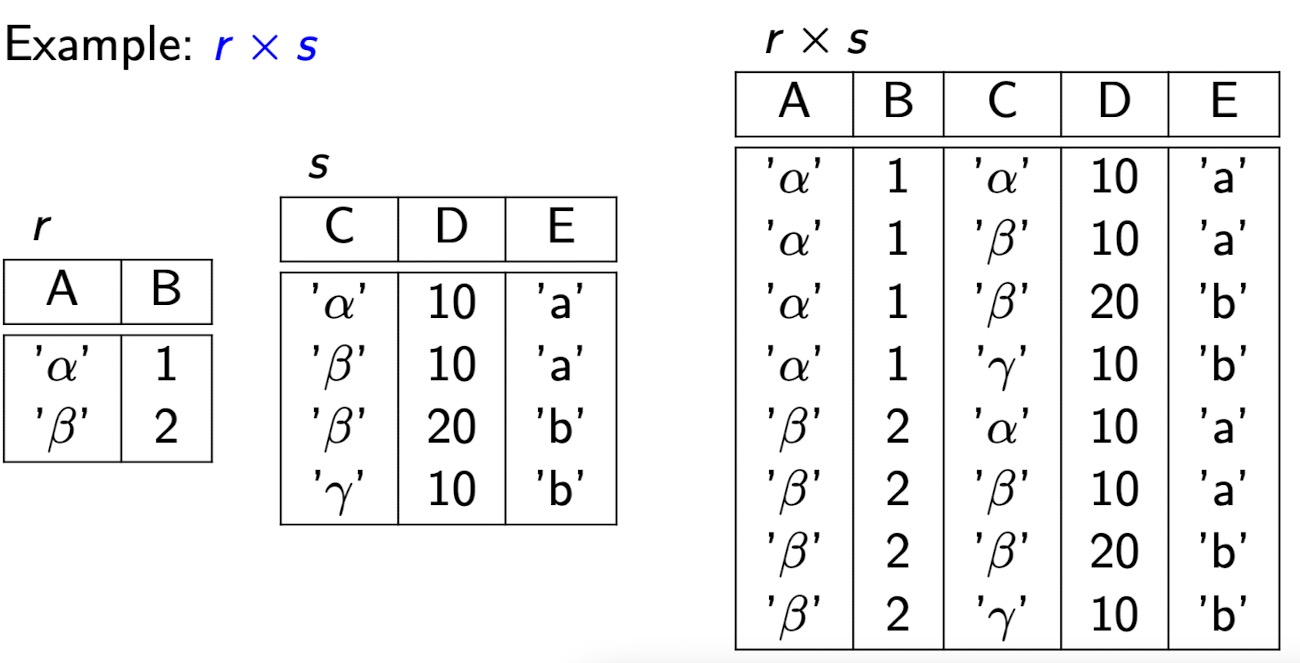
\includegraphics[width=0.6\textwidth]{images/Screenshot 2024-05-01 at 18.40.41.jpg}
\caption{Cartesian Product}
\end{figure}

\subsubsection{Rename Operator}
\begin{itemize}[label=\(\rhd\)]
    \item Allows us to name the results of relation algebra expressions by setting relation and attribute names
    \begin{itemize}[label=\(\rhd\)]
        \item $\rho_r(E)$ changes the relation name to $r$
        \item $\rho_{r(A_1,...,A_n)}(E)$ changes the relation name to $r$ and the attribute names to $A_1,...,A_k$
        \item $\rho_{(A_1,...,A_n)}(E)$ changes attribute names to $A_1,...,A_k$
    \end{itemize}
    \item Example: $\rho_{s(X,Y,U,V)}(r)$
\end{itemize}

\subsection{Additional Relational Algebra Operators}

\begin{itemize}[label=\(\rhd\)]
    \item Set intersection $\cap$
    \item Join $\bowtie$
    \item Division $\div$
    \item Assignment $\leftarrow$
\end{itemize}

These additional operators \textbf{do not add expressive power}. They just simplify queries, they could be replaced by basic operators.

\subsubsection{Set Intersection Operator}
\begin{itemize}[label=\(\rhd\)]
    \item \textbf{Notation}: $r \cap s$
    \item \textbf{Definition}: $t \in (r \cap s) \Leftrightarrow t \in r \land t \in s$
    \item Precondition:
    \begin{itemize}[label=\(\rhd\)]
        \item $r,s$ have the same arity
        \item attributes of $r$ and $s$ are compatible
    \end{itemize}
    \item Note: $r \cap s = r-(r-s)$
    \item Example: $r \cap s$
\end{itemize}

\subsubsection{Theta Join Operator}
\begin{itemize}[label=\(\rhd\)]
    \item \textbf{Notation}: $r \bowtie_\theta s$
    \item \textbf{Definition}: Let $r$ and $s$ be relations on schema $R$ and $S$, respectively. $\theta$ is a boolean condition on the attributes of $r$ and $s$
    \item $r \bowtie_\theta s$ is a relation on schema that includes all attributes from schema $R$ and all attributes from schema $S$
    \item Example: $r \bowtie_{B<X\land D = Y} \rho_{(X,Y,Z)} (s)$
\end{itemize}

\subsubsection{Natural Join Operator}
\begin{itemize}[label=\(\rhd\)]
    \item \textbf{Notation}: $r \bowtie s$
    \item \textbf{Definition}: Let $r$ and $s$ be relations on schema $R$ and $S$, respectively.
    \item $r \bowtie s$ is a relation on schema that includes all attributes from schema $R$ and all attributes from schema $S$ that do not occur in schema $R$.
    \item Joins by all matching columns!
    \item Example: $r \bowtie (s)$ [works only if attribute names are the same]
\end{itemize}

\subsubsection{Division Operator}
\begin{itemize}[label=\(\rhd\)]
    \item \textbf{Notation}: $r \div s$
    \item Suited for queries that include the phrase "for all".
    \item Let $r$ and $s$ be relations on schemas $R(A_1,...,A_m,B_1,...,B_n)$ and $S(B_1,...,B_n)$, respectively.
    \item The result of $r \div s$ is a relation with attributes $R-S=(A_1,...,A_m)$
    \item \textbf{Definition}: $t\in (r \div s) \Leftrightarrow t \in \pi_{R-S}(r) \land \forall u \in s(t\circ u \in r)$
    \begin{itemize}[label=\(\rhd\)]
        \item $t \circ u$ is the concatenation of tuples $t$ and $u$
        \item $R-S$: all attributes of schema $R$ that are not in schema $S$
    \end{itemize}
    \item Own words: $r\div s$ gives all tuples of $r$ (only those attributes that are not in $s$), where all possible combinbations with $s$ exists: 

\begin{figure}[H]
\centering
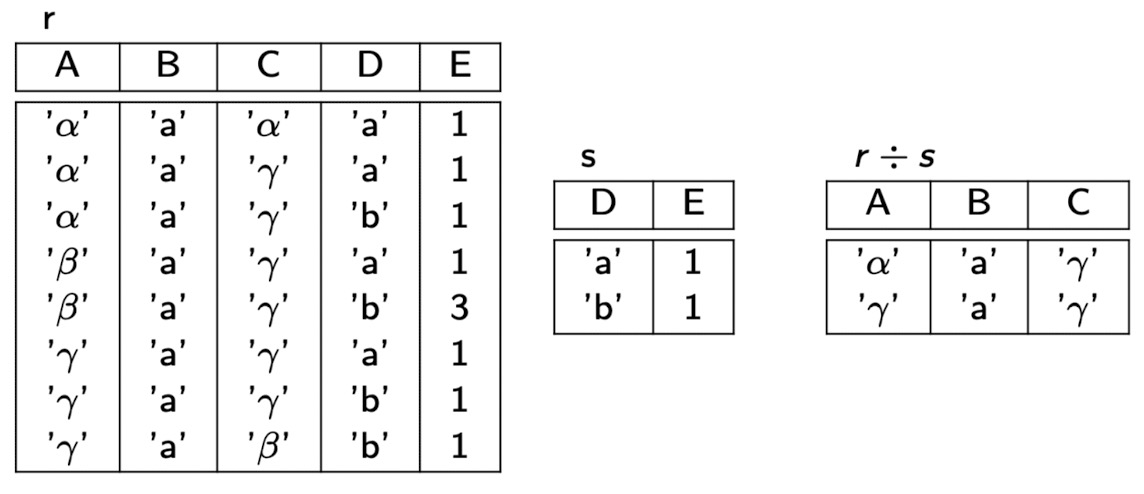
\includegraphics[width=0.6\textwidth]{images/Screenshot 2024-05-04 at 09.59.38.jpg}
\caption{Division Operator}
\end{figure}
    \begin{itemize}[label=\(\rhd\)]
        \item $'\alpha','a','\gamma'$ is in output because both 'combinations' with $s$, $'\alpha','a','\gamma','a',1$ and $'\alpha','a','\gamma','b',1$ exist already in $r$.
        \item $'\beta','a','\gamma'$ is not in output because only $'\beta','a','\gamma','a',1$ is in $r$ and $'\beta','a','\gamma','b',1$ is not
    \end{itemize}
    \item Property: 
    \begin{itemize}[label=\(\rhd\)]
        \item Let $q=r\div s$
        \item Then $q$ is the largest relation satisfying $q\times s \subseteq r$
    \end{itemize}
\end{itemize}

\subsubsection{Assignment Operator}
\begin{itemize}[label=\(\rhd\)]
    \item The assignment operator $\leftarrow$ provides a convenient way to express complex queries by breaking them up into smaller pieces
\end{itemize}

\subsection{Extended Relational Algebra Operators}

\subsubsection{Generalized Projection}
\begin{itemize}[label=\(\rhd\)]
    \item Extends the projection operation by allowing arithmetic functions to be used in the projection list
    \item Example: $\pi_{CustName, Limit - CreditBal}(credit\_info)$
\end{itemize}
\subsubsection{Aggregate Functions}
\begin{itemize}[label=\(\rhd\)]
    \item \textbf{Aggregate function} takes a collection of values and returns a single value as a result: (avg, min, max, sum, count)
    \item Example: $res \leftarrow \rho_{Res(SumC)} ( \vartheta _{sum(C)} (r))$
    \item Example: $res \leftarrow \rho_{Res(BName,SumBal)}(_{BranchName} \vartheta_{sum(Balance)}(account))$, where $BranchName$ is a grouping criteria
\end{itemize}
\subsubsection{Outer Join}
\begin{itemize}[label=\(\rhd\)]
    \item The (inner) join does not return tuples that do not have a join partner.
    \item The outer join avoids this loss of information. (By using \texttt{null} values).
    \item \textbf{Left Outer Join} preserves tuples from the left table
    \item \textbf{Right Outer Join} preserves tuples from the right table
    \item \textbf{Full Outer Join} preserves all tuples
\end{itemize}

\subsection{Modification of the Database}
Modifications are done by using the assignment operator:
\begin{itemize}[label=\(\rhd\)]
    \item Delete: $r\leftarrow r - E$
    \item Insert: $r \leftarrow r \cup E$
    \item Update: $r \leftarrow E$
\end{itemize}
Modification operations are expensive, since space for the tuples must be allocated/deallocated.
\subsection{Relation Algebra Notation in Text Terminals}

\begin{figure}[H]
\centering
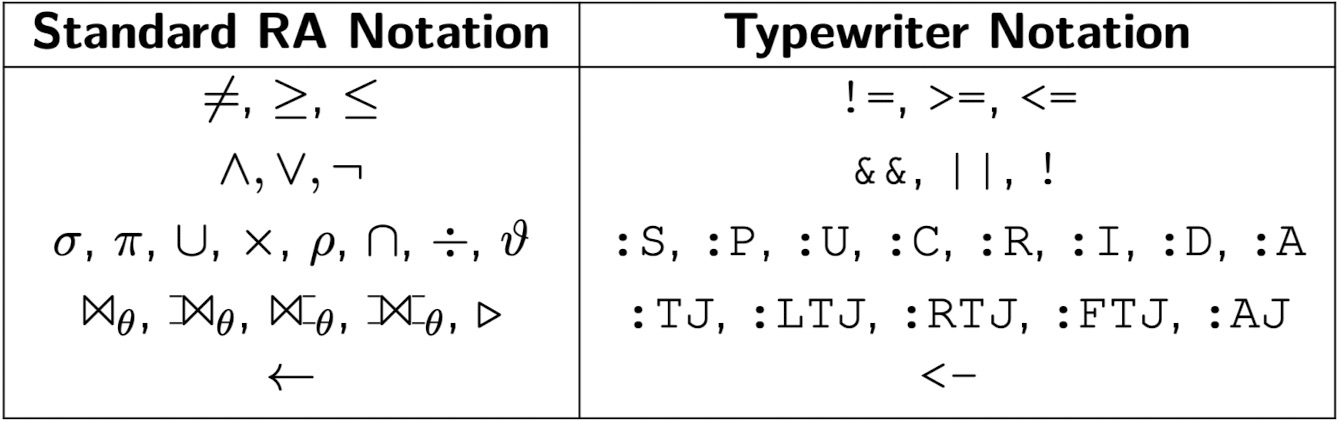
\includegraphics[width=0.6\textwidth]{images/Screenshot 2024-05-04 at 10.44.01.jpg}
\caption{Text Terminal Notation}
\end{figure}
\begin{itemize}[label=\(\rhd\)]
    \item Additional Typewriter Notation for DRC:
    \begin{itemize}[label=\(\rhd\)]
        \item $\Rightarrow=$ \texttt{=>}
        \item $\forall=$ \texttt{:F}
        \item $\exists$ \texttt{:E}
    \end{itemize}
    \item Instead of subscripts use \texttt{[ ]} brackets
    \item Replace \texttt{T} with \texttt{N} for natural joins
\end{itemize}

\subsection{Relational Calculus}

Relational calculus is a \textbf{non-procedural} or \textbf{declarative} language

\subsubsection{First Order Predicate Logic}
Syntax:
\begin{itemize}[label=\(\rhd\)]
    \item \textbf{logical symbols}: $\land, \lor, \lnot, \Rightarrow, \exists, \forall, ...$
    \item \textbf{constant}: string, number,...;
    \item \textbf{identifier}: character sequence starting with a letter
    \item \textbf{variable}: identifier starting with capital letter
    \item \textbf{predicate symbol}: identifier starting with lower case letter
    \item \textbf{built-in predicate symbol}: $=,<,>,\leq,\geq,\neq,...$
    \item \textbf{term}: constant, variable
    \item \textbf{atom}: predicate, built-in predicate; $p(t_1,...,t_n), t_1<t_2,...$ with terms $t_1,...,t_n$; predicate symbol $p$
    \item \textbf{formula}: atom, $A \land B, A \lor B, \lnot A, A \Rightarrow B, \exists XA, \forall XA, (A),... $ with formulas $A, B$; variable $X$
\end{itemize}
Terminology:
\begin{itemize}[label=\(\rhd\)]
    \item A variable is \textbf{free} is it is not quantified
    \item A variable is \textbf{bound} if it is quantified
\end{itemize}

\subsubsection{Domain Relation Calculus}
A domain relational calculus query is of the form $\{X_1,...,X_n | formula \}$, where $X_1,...,X_n$ are the only free variables in \textit{formula}
\begin{itemize}[label=\(\rhd\)]
    \item Example: To determine first and last names of all employees whose salary is above \$50,000, we write: \[
    \{FN, LN \ |\  \exists Sal(emp(FN, \_, LN, \_, Sal) \land Sal >50000) \}
    \]
\end{itemize}

\section{SQL}
\begin{itemize}
    \item SQL is based on \textbf{multisets} (or bags) rather than sets. In a multiset an element may occur multiple times.
    \begin{itemize}
        \item Reasons for not automatically removing duplicates:
        \begin{itemize}
            \item expensive to remove duplicates (sorting)
            \item for aggregation duplicates are relevant
        \end{itemize}

    \end{itemize}
    \item We write \{...\} for a set and \{\{...\}\} for a bag
\end{itemize}

\begin{table}[H]
\centering
\begin{tabular}{|c|c|c|}
    \specialrule{0.01em}{0em}{0em} 
     \textbf{SQL} & \textbf{Relational Algebra} & \textbf{Domain Relational Calculus}  \\
    \specialrule{0.01em}{0em}{0em} 
     table & relation & predicate \\
    \specialrule{0.005em}{0em}{0em} % Fine line with specified thickness and spacing
     column & attribute & argument\\
    \specialrule{0.005em}{0em}{0em}  % Fine line with specified thickness and spacing
    row & tuple & - \\
    \specialrule{0.005em}{0em}{0em}  % Fine line with specified thickness and spacing
    query & RA expression & formula \\
     \specialrule{0.01em}{0em}{0em} 
\end{tabular}
\end{table}

\subsection{Data Definition Language}

\subsubsection{Domain Types}
Domain Types in SQL:
\begin{itemize}
    \item CHAR(n): fixed length character string
    \item VARCHAR(n): character string with maximum length $n$
    \item INTEGER
    \item SMALLINT
    \item NUMERIC(p,d): Fixed point number, user-specified precision of $p$ digits, with $n$ digits to the right of decimal point
    \item REAL, DOUBLE PRECISION: Floating point and double-precision floating point numbers
    \item FLOAT(n): Floating point number, with user-specified precision of at least $n$ digits
\end{itemize}
\subsubsection{Create, dropping and altering tables}
\textbf{\underline{Create Table Construct}}
\bigskip

Example: 
\begin{lstlisting}[caption= Create Table Example]
    CREATE TABLE branch (
        BranchName CHAR(15),
        BranchCity CHAR(30),
        Assets INTEGER )
\end{lstlisting}

\textbf{\underline{Drop and Alter Table Constructs}}
\bigskip
\begin{itemize}
    \item The \textbf{drop table} command deletes the whole table from the database
    \item The \textbf{alter table} command is used to add columns to an existing table
    \begin{itemize}
        \item[] \textbf{alter table} r \textbf{add} $A$ $D$ 
    \end{itemize}
\end{itemize}


\subsubsection{Integrity constrains}

\begin{itemize}
    \item Integrity constraints guard against damage to the database
    \item Formally, an integrity constraint is a closed first order formula that must be true, i.e., that each database instance must satisfy.
    \begin{itemize}
        \item Example: $\forall B(account(\_,\_,B) \Rightarrow B<10M)$
    \end{itemize}
\end{itemize}

Integrity constraints on single relations:
\begin{itemize}
    \item \textbf{Domain Constraints}
    \begin{itemize}
        \item Domain constraints are the most elementary form of integrity constraints. They check values inserted in the database, and they check queries to ensure that the comparisons make sense.
        \item New domains can be created from existing data types
        \item Example:
        \begin{itemize}
            \item[] \begin{lstlisting}
                CREATE DOMAIN Dollars INTEGER
                CREATE DOMAIN Pounds INTEGER
            \end{lstlisting}
        \end{itemize}
        \item We cannot assign or compare a value of type Dollar to a value of type Pounds. But we can convert values: 
        \begin{itemize}
            \item[] \begin{lstlisting}
                CAST(r.Amnt/1.5 AS Pounds)
            \end{lstlisting}
        \end{itemize}
    \end{itemize}
    \item \textbf{not null}
    \begin{itemize}
        \item[] \begin{lstlisting}
            BranchName VARCHAR(15) NOT NULL
            CREATE DOMAIN Dollars INTEGER NOT NULL
        \end{lstlisting}
    \end{itemize}
    \item \textbf{primary key}
    \begin{itemize}
        \item A primary key ensures that an attribute value is not null and unique across all rows of a table. Therefore it can be used to identify a unique row in a table, and is used for query optimization
        \item Within the Create Table construct include \begin{lstlisting}
            PRIMARY KEY (CustName)
        \end{lstlisting}
    \end{itemize}
    \item \textbf{unique}
    \begin{itemize}
        \item The unique specification states that the attributes $A_1,A_2,...,A_m$ form a candidate key.
        \item Candidate keys are permitted to be null 
    \end{itemize}
    \item \textbf{check}($P$), where $P$ is a predicate over a single relation 
    \begin{itemize}
        \item Within the Create Table Construct include: \begin{lstlisting}
            CHECK (Assets >= 0)
        \end{lstlisting}
    \end{itemize}
\end{itemize}

Integrity constraints over multiple relations (Referential Integrity):
\begin{itemize}
    \item \textbf{foreign key}
    \begin{itemize}
        \item Within the Create Table Construct include:
        \begin{lstlisting}
            FOREIGN KEY (BranchN) REFERENCES branch
        \end{lstlisting}
    \end{itemize}
    \item \textbf{check}($P$), where $P$ is a predicate over multiple relations
    \item \textbf{assertion}
    \begin{itemize}
        \item An assertion is a predicate expressing a condition that the database must satisfy.
        \item An assertion in SQL takes the form
        \begin{itemize}
            \item[] \textbf{create assertion} <assertion-name> \textbf{check} <predicate>
        \end{itemize}
    \end{itemize}
\end{itemize}
\subsection{Expressions and Predicates}
\textbf{\underline{Expressions}}
\bigskip

\begin{itemize}
    \item Numeric functions: $+,-,*,/, abs(e), ceil(e), tan(e), log(e), round(e), sign(e), mod(e,f),...$
    \item Character functions:
    \begin{itemize}
        \item concatenation: 'abc' || 'de' = 'abcde'
        \item \textbf{position}('48' \textbf{in} 'another 48 hours') = 9
        \item \textbf{substring}('anothe' \textbf{from} 1 \textbf{for} 3) = 'ano'
        \item \textbf{upper}(e)
        \item \textbf{trim}(\textbf{leading} ' ' \textbf{from} ' test') = 'test
    \end{itemize}
    \item date and time functions:
    \begin{itemize}
        \item \textbf{current\_date}, \textbf{current\_time}
        \item \textbf{current\_timestamp}
        \item \textbf{current\_date} + \textbf{interval} '1' \textbf{day}
        \item \textbf{current\_date} - \textbf{date} '1990/3/18'
        \item \textbf{interval} '6' \textbf{day} - \textbf{interval} 'a' \textbf{day} = \textbf{interval} '5' \textbf{day}
     \end{itemize}
     \item type conversions:
     \begin{itemize}
         \item \textbf{cast}('48' \textbf{as integer}) = 48
         \item often "natural" type conversions are done implicitly
     \end{itemize}
     \item conditional statement:
     \begin{lstlisting}
         case
         when cond1 then result1
         ...
         when condN then resultN
         else resultX
         end
     \end{lstlisting}
     \item \textbf{coalesce}(val1,..., valN)
     \begin{itemize}
         \item returns the first value that is not null (and null if all values are equal to null)
     \end{itemize}
     \item  \textbf{nullif}(e1,e2)
     \begin{itemize}
         \item returns null if e1 and e2 are identical; useful if missing information is not represented with null; \textbf{nullif}(cost,9999)
     \end{itemize}
\end{itemize}

\textbf{\underline{Predicates}}
\bigskip

\begin{itemize}
    \item Predicates evaluate to true, false or unknown
    \item boolean connectives: \textbf{and}, \textbf{or}, \textbf{not}
    \item $=,<>, <,>,<=,>=$
    \item e \textbf{[not] between} e1 \textbf{and} e2
    \item e \textbf{is [not] null}
    \item e \textbf{in} (e1,...,eN)
    \item e1 \textbf{like} e2
    \begin{itemize}
        \item example:
        \begin{lstlisting}
            Name like '_ross%'
        \end{lstlisting}
        \item wildcards: \% 0-n characters, \_ 1 character
    \end{itemize}
\end{itemize}



\subsection{Table Expressions, Query Specifications, Query Expressions}
\textbf{\underline{Structure of SQL Queries:}}
\bigskip

\begin{figure}[H]
\centering
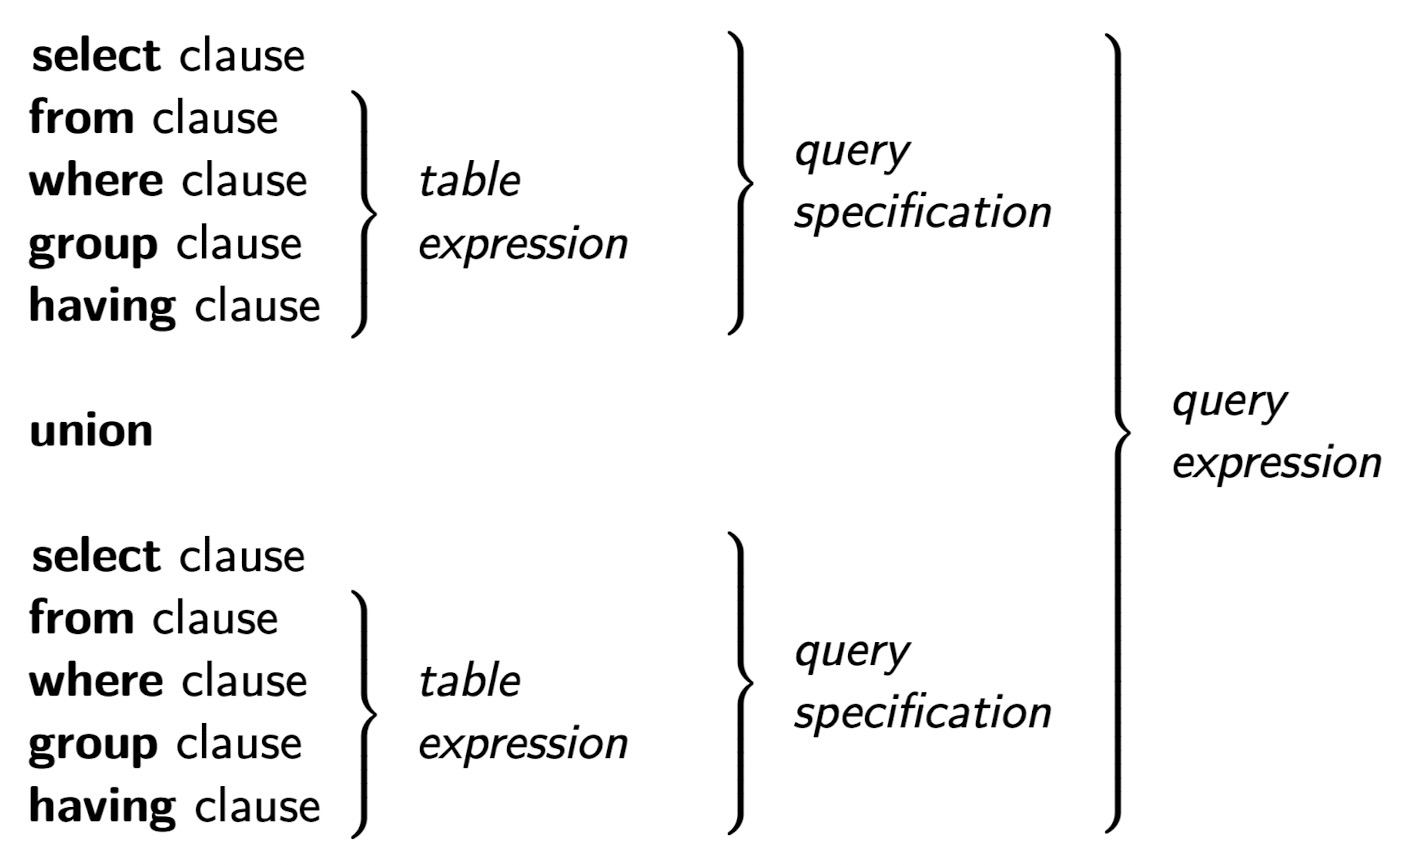
\includegraphics[width=0.6\textwidth]{images/Screenshot 2024-05-04 at 16.56.14.jpg}
\caption{SQL Structure}
\end{figure}

The result of an SQL query is a (virtual) table.

\subsubsection{The from Clause}

\begin{itemize}
    \item The \textbf{from} clause lists the table involved in the query
    \begin{itemize}
        \item Corresponds to the Cartesian product operation of the relational algebra (if multiple tables listed in from clause)
    \end{itemize}
    \item Many different joins supported
    \begin{itemize}
        \item \textbf{CROSS JOIN} = Cartesian product (implicitly also given without keyword)
        \item \textbf{Theta Join}: \quad \textbf{FROM} t1 \textbf{JOIN} t2 \textbf{ON} t1.a < t2.b
        \item \textbf{Left Outer Join}: \quad \textbf{FROM} t1 \textbf{LEFT OUTER JOIN} t2 \textbf{ON} t1.a = t2.b
        \item \textbf{Natural Join}:  \quad \textbf{FROM} t1 \textbf{NATURAL INNER JOIN} t2 
        \item \textbf{Limited Natural Join} (not all pair-wise equal columns are used for the natural join; only the ones specified in the using clause):  \quad \textbf{FROM} t1 \textbf{NATURAL INNER JOIN} t2 \textbf{USING} (name)
    \end{itemize}
\end{itemize}

\subsubsection{The where Clause}

\begin{itemize}
    \item The \textbf{where} clause specifies conditions that the result tuples must satisfy
    \item Example:
    \begin{lstlisting}
        FROM loan
        WHERE BranchName = 'Perryridge' 
            AND Amount > 1200
    \end{lstlisting}
    \item logical connectives: and, or, not
\end{itemize}

\subsubsection{The group Clause}
\begin{itemize}
    \item The \textbf{group} clause takes the table produced by the where clause and returns a grouped table
    \item Example:
    \begin{lstlisting}
        FROM account
        GROUP BY BranchName
    \end{lstlisting}
    \item The following statements work on the groups (and not on individual tuples)
\end{itemize}

\subsubsection{The having Clause}
\begin{itemize}
    \item The \textbf{having} clause takes a grouped table as input and returns a grouped table
    \item The having condition is applied to each group. Only groups that satisfy it are returned
    \item Example:
    \begin{lstlisting}
        FROM account
        GROUP BY BranchName
        HAVING COUNT(AccNr) > 1
    \end{lstlisting}
\end{itemize}

\subsubsection{The select Clause}
\begin{itemize}
    \item The \textbf{select} clause lists the columns that shall be in the result of a query
    \begin{itemize}
        \item Corresponds to the projection operation of RA
    \end{itemize}
    \item To force the elimination of duplicates, insert the keyword \textbf{distinct} after select
    \item In the select clause aggregate functions can be used:
    \begin{itemize}
        \item avg, min, max, sum, count
    \end{itemize}
\end{itemize}

\subsubsection{Derived Tables}
\begin{itemize}
    \item SQL allows a query expression to be used in the \textbf{from} clause
    \item Example:
    \begin{lstlisting}
        SELECT BranchName, AvgBalance
        FROM ( SELECT BranchName AVG(Balance)
               FROM account
               GROUP BY BranchName
             ) AS branchAvg(BranchName, AvgBalance)
        WHERE AvgBalance > 1200
    \end{lstlisting}
\end{itemize}

\subsubsection{Query Expressions}
\begin{itemize}
    \item The set operations \textbf{union}, \textbf{intersect}, and \textbf{except} operate on tables and correspond to the relational algebra operations $\cup, \cap, -$
    \item Each automatically removes duplicates, to preserve duplicates add \textbf{all} after operator
\end{itemize}

\subsection{Subqueries, Duplicates, Null Values}

\subsubsection{Subqueries}

\begin{itemize}
    \item A \textbf{subquery} is a \textbf{query expression} that is nested within another query expression.
    \item Example:
    \begin{lstlisting}
        SELECT X FROM p WHERE X IN (SELECT Y FROM q)
    \end{lstlisting}
    \item[\textbf{!}] Semantics/evaluation: For each tuple of p evaluate the subquery and check if X is in the result table computed by the subquery
    \item The \textbf{exists} construct returns the value \textbf{true} if the argument subquery is nonempty
    \begin{itemize}
        \item[\textbf{!}] Use \textbf{exists} instead of \textbf{in, all, any, some}
    \end{itemize}
\end{itemize}

\subsubsection{Duplicates}

SQL duplicate semantics:\\

\quad \textbf{select} $A_1,A_2,...,A_n$ \

\quad \textbf{from} $r_1, r_2,...,r_m$ \

\quad \textbf{where} $P$\\

is equivalent to the \textit{multiset} version of the expression: \[
\pi_{A_1,A_2,...,A_n}(\sigma_P (r_1 \times r_2 \times ... \times r_m))
\]

\subsubsection{Null Values}
\begin{itemize}
    \item The  predicate \textbf{is null} can be used to check for null values.
    \item Any comparison with \textit{null} returns unknown
    \begin{itemize}
        \item Example: $5<null$ or $null<>null$ or $null=null$ 
    \end{itemize}
    \item All aggregate operations, expect \textbf{count(*)}, ignore tuples with null values on the aggregated columns. 
    \begin{itemize}
        \item Arithmetic operations like $7+ null = null$, thus they do not ignore null values
    \end{itemize}
\end{itemize}

\subsubsection{Ordering}

\begin{itemize}
    \item \textbf{ORDER BY} CustName => orders the result table alphabetically (ascending = default)
    \item \textbf{ORDER BY} CustName \textbf{DESC} => in descending order
\end{itemize}

\subsection{Modification of the Database}

\subsubsection{Insertions}
\begin{lstlisting}
    INSERT INTO account
        VALUES ('A-9732', 'Perryridge', 1200)
\end{lstlisting}

\subsubsection{Deletions}
\begin{lstlisting}
    DELETE FROM account
    WHERE BranchName = 'Perryridge'
\end{lstlisting}
\subsubsection{Updates}
\begin{lstlisting}
    UPDATE account
    SET Balance = Balance * 1.06
    WHERE Balance > 10000

    UPDATE account 
    SET Balance = Balance * 1.05
    WHERE Balance <= 10000
\end{lstlisting}
Here order matters! $\Rightarrow$ Better use the \textbf{case} statement 
\begin{lstlisting}
    UPDATE account
    SET Balance = CASE 
                    WHEN Balance <= 10000
                    THEN Balance * 1.05
                    ELSE Balance * 1.06
                  END
\end{lstlisting}   

\subsection{Views and Recursion}

\subsubsection{Purpose of views}

\subsubsection{Creation and use of views}

\subsubsection{Handling views in the DBMS}

\subsubsection{Temporary Views}


\subsection{User Defined Functions}

\section{Relational Database Design}
\subsection{Relational Database Design Guidelines}

\subsubsection{Goals of Relational Database Design}
The goal of relational database design is to find a good collection of relation schemas. The main problem is to find a good grouping of the attributes into relation schemas.\\
We have a good collection of relation schemas if we:
\begin{itemize}[label=\(\rhd\)]
    \item Ensure a simple semantics of tuples and attributes
    \item Avoid redundant data
    \item Avoid update anomalies
    \item Avoid null values as much as possible
    \item Ensure that exactly the original data is recorded and (natural) joins do not generate spurious tuples
\end{itemize}\

\textbf{Guideline 1:} Each tuple in a relation should only represent one entity or relationship instance \

\textbf{Guideline 2:} Design a schema that does not suffer from insertion, deletion and update anomalies.\

\textbf{Guideline 3:} Relations should be designed such that their tuples will have as few NULL values as possible; attributes that are NULL shall be placed in separate relations (along with the primary key)\

\textbf{Guideline 4:} Relations should be designed such that no spurious (i.e., wrong) tuples are generated if we do a natural join of the relations

\subsection{Functional Dependencies}
Reminder Key Constraints: \ref{keyConstraints}


\subsubsection{Definition}

Functional dependencies (FDs) are used to specify \textit{formal measures} of the goodness of relation designs. FDs and keys are used to define \textbf{normal forms} for relations. Functional Dependencies are \textbf{constraints} that are derived from the \textit{meaning} and \textit{interrelationships} of the attributes.\\

A set of attributes X \textit{functionally determines} a set of attributes Y if the value of X determines a unique value for Y. \[X \rightarrow Y\]

A functional dependency $X\rightarrow Y$ is \textbf{trivial} iff $Y\subseteq X$: \quad $(\underset{X}{FN,LN} \rightarrow \underset{Y}{FN})$ \label{trivial}\\

\begin{itemize}[label=\(\rhd\)]
    \item A FD constraint must hold on \textit{every} relation instance r(R)
    \item If K is a candidate key of R, the K functionally determines all attributes in R (since we never have two distinct tuples with $t_1[K]=t_2[K]$ 
\end{itemize}



\subsubsection{Armstrong's inference rules}
\begin{itemize}[label=\(\rhd\)]
    \item Given a set of FDs $F$, we can \textbf{infer} additional FDs that hold whenever the FDs in $F$ hold
    \item Armstrong's inference rules:
    \begin{itemize}[label=\(\rhd\)]
        \item Reflexivity: $Y\subseteq X \models X\rightarrow Y$
        \item Augmentation: $X \rightarrow Y \models XZ \rightarrow YZ$
        \item Transitivity: $X\rightarrow Y, Y \rightarrow Z \models X \rightarrow Z$
    \end{itemize}
    \item Armstrong's inference rules are \textbf{sound} and \textbf{complete}
    \item Additional inference rules that are useful:
    \begin{itemize}[label=\(\rhd\)]
        \item Decomposition: $X\rightarrow YZ \models X \rightarrow Y, X \rightarrow Z$
        \item Union: $X \rightarrow Y, X \rightarrow Z \models X \rightarrow YZ$
        \item Pseudotransitivity: $X \rightarrow Y, WY \rightarrow Z \models WX \rightarrow Z$
    \end{itemize}
\end{itemize}

\subsubsection{Closure and minimal cover}
\begin{itemize}[label=\(\rhd\)]
    \item The \textbf{closure} of a set t $F$ of FDs is the set $F^{+}$ of all FDs that can be inferred from $F$
    \item The \textbf{closure} of a set of attributes $X$ with respect to $F$ is the set $X^+$ of all attributes that are functionally determined by $X$
    \item Two sets of FDs $F$ and $G$ are \textbf{equivalent} if:
    \begin{itemize}[label=\(\rhd\)]
        \item Every FD in $F$ can be inferred from $G$, and
        \item Every FD in $G$ can be inferred from $F$
        \item Hence, $F$ and $G$ are equivalent if $F^+ = G^+$
    \end{itemize}
    \item Definition: $F$ \textbf{covers} $G$ if every FD in $G$ can be inferred from $F$ (i.e., if $G^+ \subseteq F^+$)
    \item A set of FDs is \textbf{minimal} if it satisfies the following conditions:
    \begin{enumerate}
        \item No pair of FDs has the same left-hand side 
        \item We cannot remove any dependency from $F$ and have a set of dependencies that is equivalent to $F$ 
        \item We cannot replace any dependencies $X\rightarrow A$ in $F$ with a dependency $Y\rightarrow A$, where $Y\subset X$ and still have a set of dependencies that is equivalent to $F$
    \end{enumerate}
\end{itemize}

\subsection{Normal Form}
\begin{itemize}[label=\(\rhd\)]
    \item \textbf{Normalization}: The process of decomposing bad relations by breaking up their attributes into smaller relations that satisfy the normal forms. 
    \item A normalized database consists of a good collection of relation schemas
    \item The database designers \textit{need not} normalize to the highest possible normal form
    \begin{itemize}[label=\(\rhd\)]
        \item usually they choose 3NF, BCNF or 4NF 
        \item controlled redundancy is OK/good
    \end{itemize}
\end{itemize}

\subsubsection{First Normal Form (1NF)}
Dissallows: \begin{itemize}[label=\(\rhd\)]
    \item composite attributes
    \item multivalued attributes 
    \item nested relations: attributes whose values for an \textit{individual tuple} are relations 
\end{itemize}
Remedy to get 1NF: Form new relations for each multivalued attribute or nested relation

\subsubsection{Second Normal Form (2NF)}
\begin{itemize}[label=\(\rhd\)]
    \item A relation schema R is in \textbf{second normal form (2NF)} iff each attribute not contained in a candidate key is not partially functional dependent on a candidate key of R. 
    \item An attribute is \textit{partially functional dependent} on a candidate key if it is functionally dependent on a proper subset of the candidate key
    \item Example: given candidate key SSN, PNum the FD $SSN \rightarrow EName$ would violate 2NF as EName is partially functional dependent on the candidate key (or fully funtional dependent on the subset SSN of the candidate key)
    \item \textbf{Remedy}: Decompose and set up a new relation for each partialy key with its dependent attributes. Keep a relation with the original key and any aatributes that are functionally dependent on it. 
\end{itemize}

\subsubsection{Third Normal Form (3NF)}

\begin{itemize}[label=\(\rhd\)]
    \item A relation schema R is in \textbf{third normal form (3NF)} iff for all $X\rightarrow A \in F^+$ at least \textbf{one} of the following holds:
    \begin{itemize}[label=\(\rhd\)]
        \item $X\rightarrow A$ is trivial \ref{trivial}
        \item X is a superkey for R
        \item A is contained in a candidate key of R
    \end{itemize}
    \item Intuition: "Each non-key attribute must describe the key, the whole key, and nothing but the key."
    \item A relation that is in 3NF is also in 2NF 
\end{itemize}

\subsubsection{Boyce-Codd Normal Form (BCNF)}
\begin{itemize}[label=\(\rhd\)]
    \item A relation schema R is in \textbf{Boyce-Codd Normal Form (BCNF)} iff for all $X\rightarrow A \in F^+$ at least one of the following holds:
    \begin{itemize}[label=\(\rhd\)]
        \item $X\rightarrow A$ is trivial
        \item X is a superkey of R  
    \end{itemize}
    \item Remedy to get BCNF: split relation
\end{itemize}

\subsection{Properties of Decomposition and Normalization Algorithm}
\begin{itemize}[label=\(\rhd\)]
    \item Relational database design by decomposition:
    \begin{itemize}[label=\(\rhd\)]
        \item Universal Relation Schema: A relation schema $R(A_1,A_2,,...,A_n)$ that includes all attributes of the database
        \item Decomposition: decompose the universal relation schema R into a set of relation schemas $D=R1,R2,...,Rm$ by using the functional dependencies
        \item Additional conditions:
        \begin{itemize}[label=\(\rhd\)]
            \item Each attribute in R will appear in at least one relation schema Ri in the decomposition so that no attributes are lost
            \item Have each individual relation Ri in the decomposition D in 3NF (or higher)
            \item \textbf{Lossless join decomposition}: ensures that the decomposition does not introduce wrong tuples when relations are joined together [must have]
            \item \textbf{Dependency preservation}: ensures that all functional dependency can be checked by considering individual relations Ri only [nice to have]
        \end{itemize}
    \end{itemize}
\end{itemize}

\subsubsection{Dependency Preservation}
\begin{itemize}[label=\(\rhd\)]
    \item Given a set of dependencies $F$ on $R$, the \textbf{projection} of $F$ on Ri, denoted by $F|Ri$ where $attr(Ri)$ is a subset of $attr(R)$, is the set of dependencies $X\rightarrow Y$ in $F^+$ such that the attributes in $X \cup Y$ are all contained in $attr(Ri)$
    \item Hence, the projection of $F$ on each relation schema $Ri$ in the decomposition $D$ is the set of functional dependencies in $F^+$, the closure of $F$. such that all their left- and right-hand side attributes are in $attr(Ri)$
    \item Dependency Preservation:
    \begin{itemize}[label=\(\rhd\)]
        \item A decomposition $D=R1,R2,...,Rm$ of R is \textbf{dependency-preserving} with respect to F if the union of the projections of F on each Ri in D is equivalent to F; that is \[
        (F|R1 \cup ...\cup F|Rm)^+ = F^+
        \]
    \end{itemize}
    \item It is always possible to find a dependency-preserving decomposition such that each relation is in 3NF
    \item It is not always possible to find a dependency-preserving decomposition such that each relation is in BCNF
\end{itemize}
\subsubsection{Lossless Join Decomposition}
\begin{itemize}[label=\(\rhd\)]
    \item A decomposition $D=R1,R2,...,Rm$ of R is a \textbf{loss less join decomposition} with respect to the set of dependencies $F$ on $R$ if, for every relation instance $r$ of $R$ that satisfies $F$, the following holds: \[
    \pi_{R1}(r) \bowtie ... \bowtie \pi_{attr(Rm)}(r)=r
    \] (join of the pieces gives the original relation
    \item R1 and R2 form a lossless join decomposition of R with respect to a set of functional dependencies F iff 
    \begin{itemize}[label=\(\rhd\)]
        \item $(R1 \cap R2) \rightarrow (R1-R2)$ is in $F^+$ or
        \item $(R1 \cap R2) \rightarrow (R2-R1)$ is in $F^+$
    \end{itemize}
    \item Example: Consider $R(A,B,C)$, $F=\{AB\rightarrow C, C \rightarrow B\}$, $R1(A,C), R2(B,C)$. Is $R1, R2$ a lossless decomposition of R?
    \begin{itemize}[label=\(\rhd\)]
        \item $(R1 \cap R2) \rightarrow (R1-R2) \Rightarrow C \rightarrow A$. This is not in $F^+$
        \item $(R1 \cap R2) \rightarrow (R2-R1) \Rightarrow C \rightarrow B$. This is in $F^+$ 
        \item R1, R2 is thus lossless a decomposition of R
    \end{itemize}
\end{itemize}

\subsubsection{BCNF Normalization Algorithm}
\begin{algorithm}
\caption{Decompose relation schema into BCNF}
\begin{algorithmic}[1] % The number [1] ensures lines are numbered
\State Set $D := \{R\}$
\While{\textit{a relation schema $Q$ in $D$ is not in BCNF}}
    \State find a functional dependency $X \rightarrow Y$ in $Q$ that violates BCNF;
    \State replace $Q$ in $D$ by two relation schemas $(Q - Y)$ and $(X \cup Y)$;
\EndWhile
\end{algorithmic}
\end{algorithm}
\quad \textit{Assumption: No null values are allowed for the join attributes}\\
The result is a lossless join decomposition. The resulting schemas do not necessarily preserve all dependencies.

\subsection{Multivalued Dependencies, 4NF}
\textbf{Definition:}
\begin{itemize}[label=\(\rhd\)]
    \item A \textbf{multivalued dependency (MVD)} $X \twoheadrightarrow Y$ on relation schema $R$, where $X$ and $Y$ are both subsets of $R$, specifies the following constraint on any relation instance $r$ of $R$:\\
    If two tuples $t_1$ and $t_2$ exist in $r$ such that $t_1[X]=t_2[X]$, then two tuples $t_3$ and $t_4$ should also exist in $r$ with the following properties, where we use $Z$ to denote $(R-(X\cup Y))$:
    \begin{itemize}[label=\(\rhd\)]
        \item $t_3[X]=t_4[X]=t_1[X]=t_2[X]$
        \item $t_3[Y]=t_4[Y]=t_1[Y]=t_2[Y]$
        \item $t_3[Z]=t_4[Z]=t_1[Z]=t_2[Z]$
    \end{itemize}
    \item A MVD $X \twoheadrightarrow Y$ for $R$ is called a \textbf{trivial MVD} if $Y \subseteq X$ or $X\cup Y = attr(R)$
\end{itemize}

\textbf{Inference Rules for Functional and Multivalued Dependencies}:
\begin{itemize}[label=\(\rhd\)]
    \item reflexivity FDs: $X\supseteq Y \models x \rightarrow Y$
    \item augmentation FDs: $X\rightarrow Y \models XZ \rightarrow YZ$
    \item transitivity FDs: $X\rightarrow Y, Y \rightarrow Z \models X \rightarrow Z$
    \item complementation: $X \twoheadrightarrow Y \models X \twoheadrightarrow (R-(X\cup Y))$
    \item augmentation MVDs: $X\twoheadrightarrow Y, W \supseteq Z \models WX \twoheadrightarrow YZ$
    \item transitivity MVDs: $X \twoheadrightarrow Y, Y \twoheadrightarrow Z \models X \twoheadrightarrow (Z-Y)$
    \item replication: $X\rightarrow Y \models X \twoheadrightarrow Y$
    \item coalescing: $X \twoheadrightarrow Y, \exists W(W\cap Y = \emptyset, W \rightarrow Z, Y \supseteq Z) \models X \rightarrow Z$ 
\end{itemize}


\subsubsection{Fourth Normal Form (4NF)}

\textbf{Definition:}
\begin{itemize}[label=\(\rhd\)]
    \item A relation schema $R$ with a set of functional and multivalued dependencies F is in \textbf{4NF} iff, for every multivalued dependency $X \twoheadrightarrow Y$ in $F^+$ at least one of the following holds:
    \begin{itemize}[label=\(\rhd\)]
        \item $X\twoheadrightarrow Y$ is trivial
        \item X is a superkey for $R$
    \end{itemize}
    \item If a relation is not in 4NF because of the MVD $X \twoheadrightarrow Y$ we decompose R into $R1(X\cup Y)$ and $R2(R-Y)$
    \item Such a decomposition is lossless
\end{itemize}

\subsection{Summary}
\begin{itemize}[label=\(\rhd\)]
    \item Relational database design goals: eliminate redundancy
    \item Main concept: functional dependencies
    \item Functional dependencies:
    \begin{itemize}[label=\(\rhd\)]
        \item Definition
        \item Armstrong's inference rules: reflexivity, augmentation, transitivity
        \item equivalence of sets of FDs
        \item minimal sets of FDs
    \end{itemize}
    \item Approach: Start with all attributes in a single relation and decompose it vertically until all functional dependencies are acceptable
    \item Normal forms based on candidate keys and FD
    \begin{itemize}[label=\(\rhd\)]
        \item 1NF, 2NF, 3NF, BCNF
    \end{itemize}
    \item BCNF normalization algorithm 
    \item Dependency Preservation
    \begin{itemize}[label=\(\rhd\)]
        \item always possible for 3NF; not always possible for BCNF
    \end{itemize}
    \item Lossless Join Decomposition
    \begin{itemize}[label=\(\rhd\)]
        \item always required
    \end{itemize}
    \item Multivalued Dependencies, 4NF
\end{itemize}

\section{Conceptual Database Design}
\subsection{Entities, Entity Types, Entity Sets, Attributes}
\subsubsection{Entities} 
\subsubsection{Entity Types}
\subsubsection{Entity Sets}
\subsection{Attributes}

\subsection{Relationships, Relationship Types, Relationship Sets}
\subsubsection{Strucutral Constraints on Relationships}
\subsubsection{Recursive Relationships}
\subsubsection{Attributes of Relationships}

\subsection{Weak Entities, N-ary Relationships}
\subsubsection{Weak Entities}
\subsubsection{N-ary Relationships}

\subsection{Subclasses and Superclasses}
\subsubsection{Disjointness Constraint}
\subsubsection{Completeness Constraint}

\subsection{ER-to-Relational Mapping Algorithm}
\subsubsection{Mapping an ER Model to a Relational Model}


\section{Physical Database Design}
\subsection{Disk Storage and Files}
\subsubsection{Physical Storage Media}
\subsubsection{Accessing the Storage}
\subsubsection{Organization of Files}

\subsection{Index Structures}
\subsubsection{Types of Indexes}
\subsubsection{B+ Tree}
\subsubsection{Hashing}
\subsubsection{Index Definition in SQL}





\section{Query Processing and Query Optimization}
\subsection{Query Processing}
\subsubsection{Sorting, Partitioning}
\subsubsection{Selection, Join}

\subsection{Query Optimization}
\subsubsection{Cost estimation}
\subsubsection{Rewriting of relational algebra expression}
\subsubsection{Rule- and cost-based query optimization}



\section{Transaction Processing}
\subsection{Transactions}
\subsubsection{Transaction States}
\subsubsection{ACID Properties}
\subsubsection{Schedules}
\subsubsection{Serializability}
\subsubsection{Recoverability}

\subsection{Concurrency Control}
\subsubsection{Lock-Based Protocols}
\subsubsection{Pitfalls of Lock-Based Protocols}
\subsubsection{Two-Phase Locking (2PL)}
\subsubsection{Transactions in SQL}
\subsubsection{Transactions in DBMSs}

\subsection{Recovery System}
\subsubsection{Log-Based Recovery}
\subsubsection{Deferred DB Modifications}
\subsubsection{Immediate DB Modifications}
\subsubsection{Checkpoints}

\end{document}
